\section{Auswertung}
\label{sec:Auswertung}
\begin{figure}
	\centering
	\caption{Die Temperaturdifferenz $T2-T1$ bei dem breitem Messingstab gegen die vergangene Zeit $t$ aufgetragen.}
	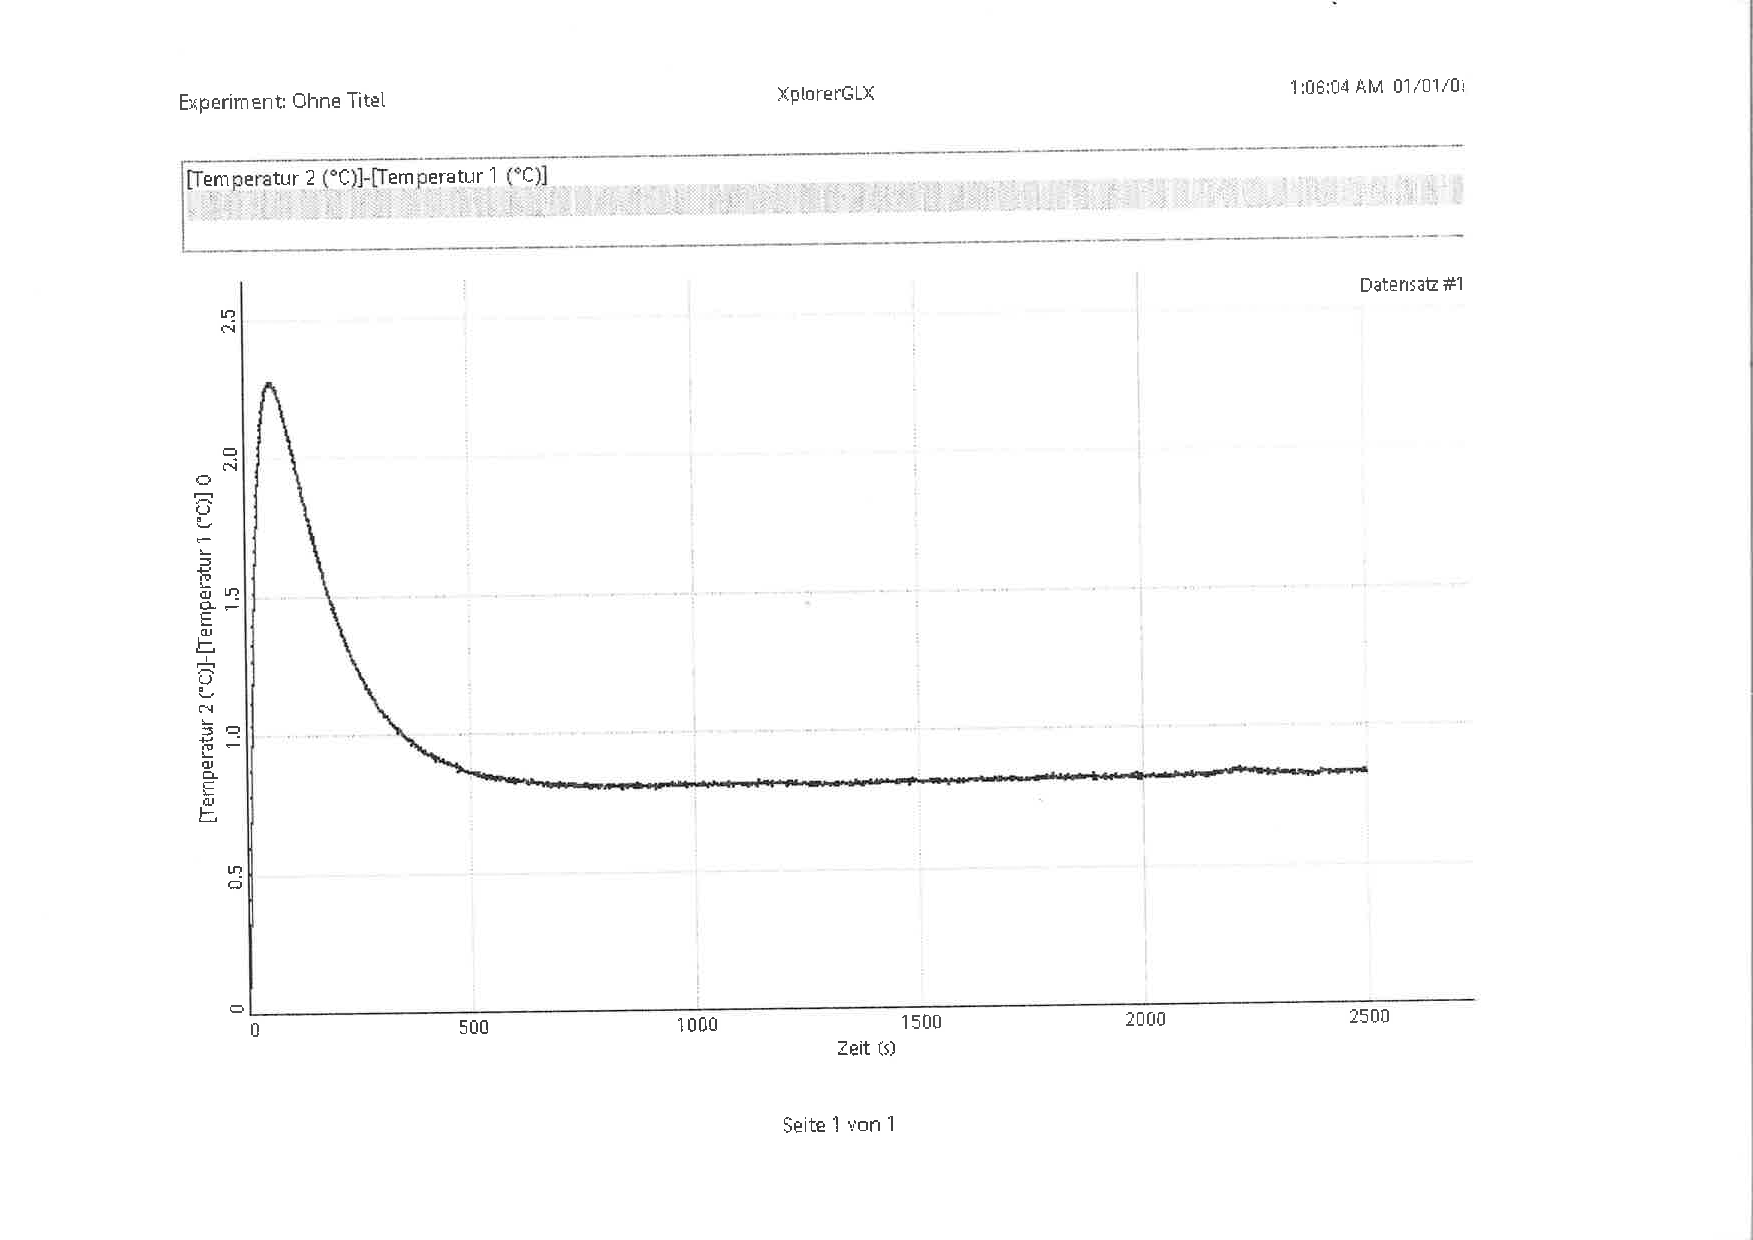
\includegraphics[width=\linewidth-70pt,height=\textheight-70pt,keepaspectratio]{content/Bilder/T2-T1-rotated.pdf}
	\label{fig:Graph3}
\end{figure}
\begin{table}
	\centering
	\caption{Der nach Formel \eqref{eq:form1} berechnete Wärmestrom $\frac{\Delta Q_{21}}{\Delta t}$ nach der Zeit $t$ und die aus \ref{fig:Graph3} entnommene Temperaturdifferenz $T2-T1$ bei dem breitem Messingstab.}
	\input{./build/tabT21.tex}
\end{table}
\begin{figure}
	\centering
	\caption{Die Temperaturdifferenz $T7-T8$ bei dem Edelstahlstab gegen die vergangene Zeit $t$ aufgetragen.}
	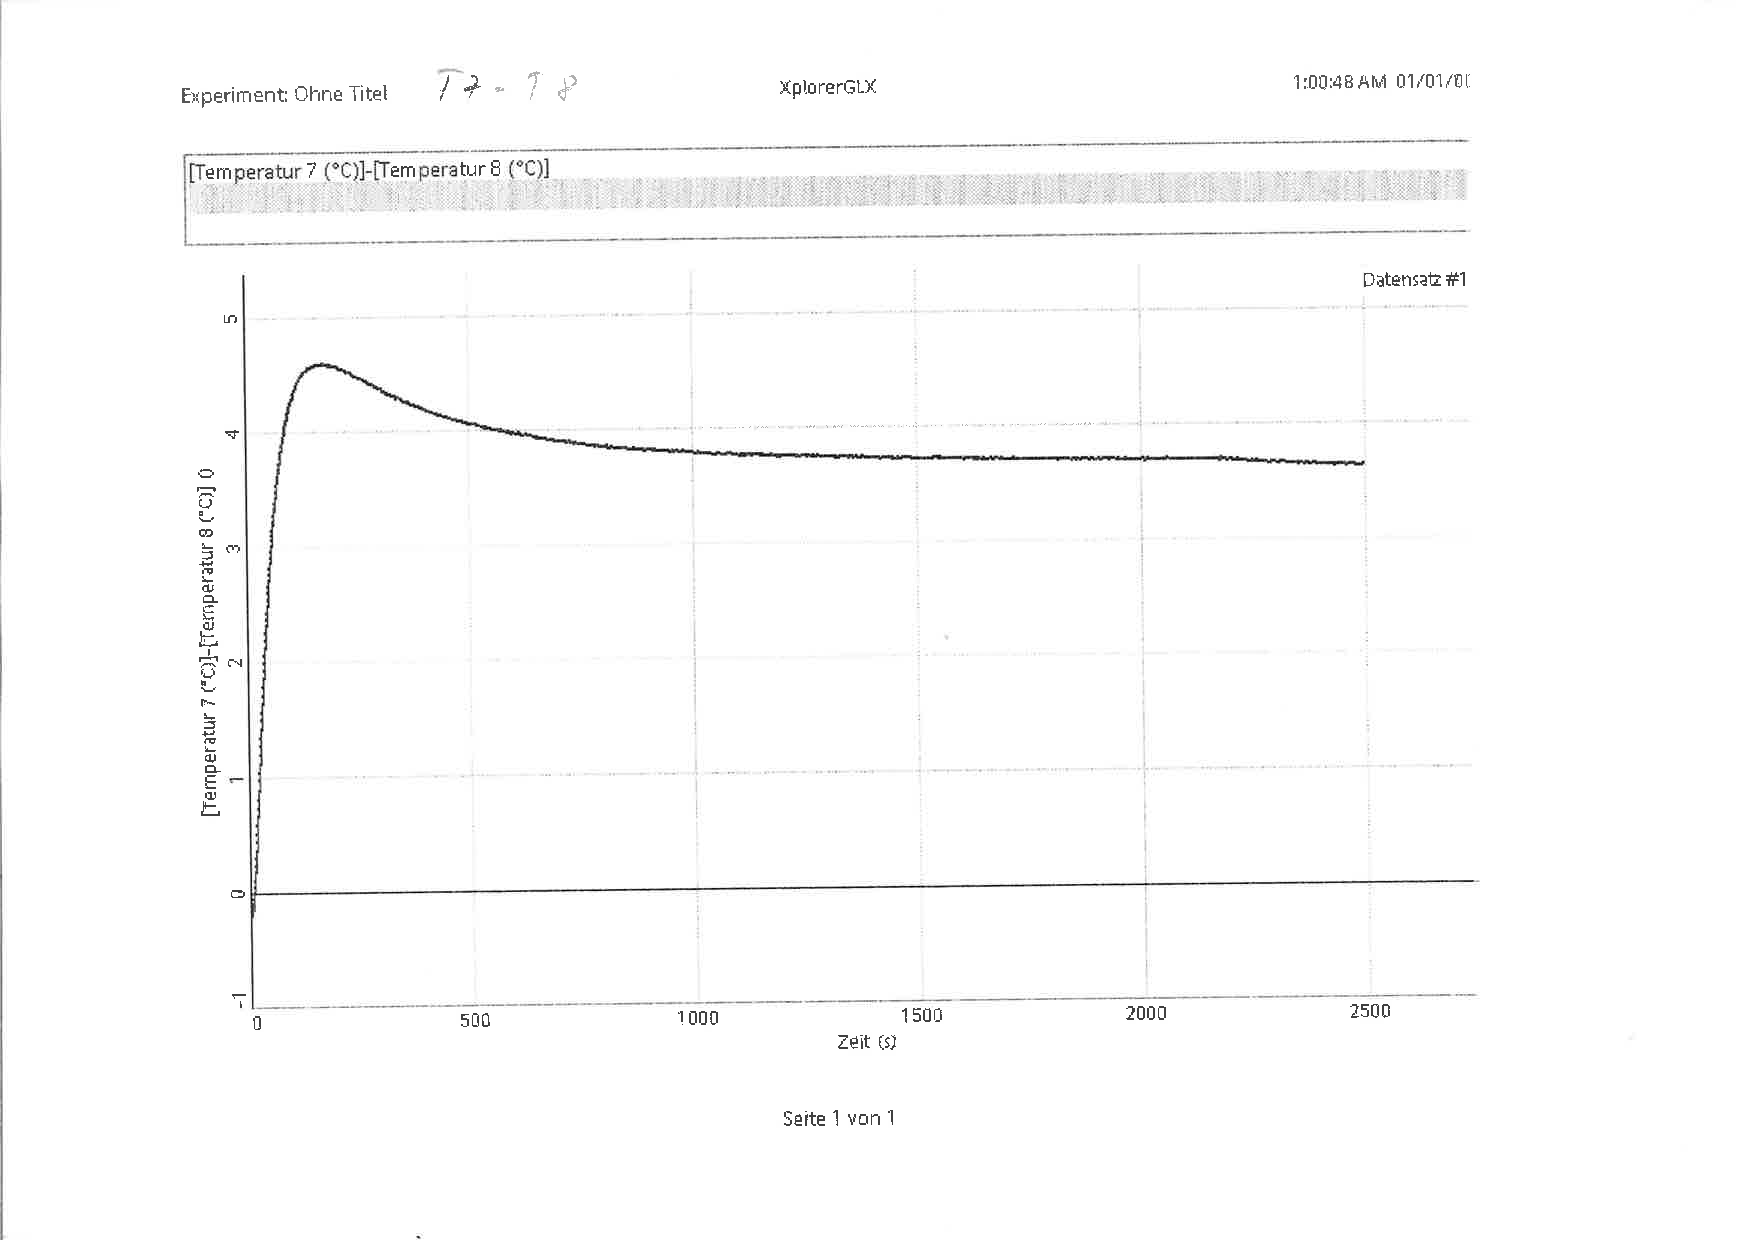
\includegraphics[width=\linewidth-70pt,height=\textheight-70pt,keepaspectratio]{content/Bilder/T7-T8-rotated.pdf}
	\label{fig:Graph4}
\end{figure}
\begin{table}
	\centering
	\caption{Der nach Formel \eqref{eq:form1} berechnete Wärmestrom $\frac{\Delta Q_{78}}{\Delta t}$ nach der Zeit $t$ und die aus \ref{fig:Graph4} entnommene Temperaturdifferenz $T7-T8$ bei dem Edelstahlstab.}
	\input{./build/tabT78.tex}
\end{table}